\section{GAN architecture}
\label{sec:gan_architecture}

Our texture and label maps are generated in multiple steps, where each step is an image-to-image transformation, implemented with a GAN. Traditional image-to-image GANs such as Pix2Pix~\cite{pix2pix} can learn a wide range of image-to-image transformations, but the variation of outputs that can be generated for a given input is limited. Since we aim to generate multiple different output styles for a given input, we base our GAN architecture on the recently introduced BicycleGAN architecture~\cite{zhu2017multimodal}, which explicitly encodes the style in a low-dimensional \emph{style space} and allows outputs to be generated with multiple styles. In this section, we briefly recap the BicycleGAN setup and describe our modifications.

Image-to-image GANs train a generator function,
%
\begin{equation}
\label{eq:gan_function}
B = G(A,Z): \mathbb{R}^n \times \mathbb{R}^k \rightarrow \mathbb{R}^n,    
\end{equation}
%
that transforms an input image $A$ to an output image $B$. For example, $A$ might be an image containing color-coded facade labels, such as windows, and $B$ a corresponding facade texture. The second input $Z$ is a vector of latent variables that describe properties of the output image that are not given by the input image, such as the wall color. We call $Z$ the \emph{style vector} and the space containing $Z$ the \emph{style space} $\mathcal{Z}$. The embedding of properties into this space is learned by the generator during training. Typically, $Z$ is chosen to be random during training and evaluation, effectively randomizing the style.

The generator's goal is to approximate some desired but unknown joint distribution $p(A,B)$ by training it with known samples from this distribution, in the form of two datasets $\mathcal{A}$ and $\mathcal{B}$ of matching input/output pairs. For example, $p(A,B)$ may be the distribution of matching pairs of facade labels and facade textures. During generator training, the difference between the generated distribution $p(A,G(A,Z))$ and the desired unknown distribution $p(A,B)$ is measured in an adversarial setup, where a \emph{discriminator} function $D$ is trained to distinguish between samples from the two distributions, with the following cross-entropy classification loss:
\begin{equation}
\begin{aligned}
\label{eq:loss_gan_d}
    \mathcal{L}^D_{\textrm{GAN}}(G,D) =\ & \mathbb{E}_{A,B \sim p(A,B)} \bigl[-\log D(A,B)\bigr]\ + \\
    & \mathbb{E}_{A,B \sim p(A,B),\ Z \sim p(Z)}\bigl[-\log \left(1-D(A,G(A,Z))\right)\bigr],
\end{aligned}
\end{equation}
where $p(Z) = \mathcal{N}(0,I)$ is the prior over style vectors, defined to be a standard normal distribution. The generator is trained to output samples that are misclassified by the discriminator as being from the desired distribution:
\begin{align}
\label{eq:loss_gan_g}
    \mathcal{L}^G_{\textrm{GAN}}(G,D) = \mathbb{E}_{A,B \sim p(A,B),\ Z \sim p(Z)}\bigl[-\log D(A,G(A,Z))\bigr].
\end{align}
Additionally, an L1 or L2 loss term between the generated output and the ground truth is usually included:
\begin{align}
\label{eq:loss_gan_l1}
    \mathcal{L}_{\textrm{L1}}(G) = \mathbb{E}_{A,B \sim p(A,B),\ Z \sim p(Z)}\bigl\|B-G(A,Z)\bigr\|_1.
\end{align}

In general, the conditional distribution $p(B|A)$ for a fixed $A$ may be a multi-modal distribution with large variance; for example, there is a wide range of possible facade textures for a given facade label image. However, previous work~\cite{pix2pix} has shown that in typical image-to-image GAN setups, the style vector $Z$ is largely ignored, resulting in a generator output that is almost fully determined by $A$ and restricting $p(B|A)$ to have low variance. To solve this problem, BicycleGAN uses an \emph{encoder} $E$ that obtains the style from an image and combines additional loss terms introduced in previous works~\cite{Donahue:2016:afl,Dumoulin:2016:ali,vae_gan} to ensure that the style is not ignored by the generator.

\begin{figure}[t]
    \centering
    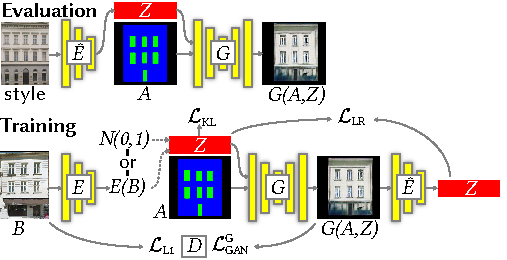
\includegraphics[width=\columnwidth]{images/gan.pdf}
    \caption{GAN architecture. The setup used during evaluation is shown in the top row, and the training setup is shown in the bottom row. Dotted lines denote random sampling.}
    \label{fig:gan}
\end{figure}

First, based on ideas from Variational Autoencoders~\cite{vae}, the encoder outputs a distribution $E(B)$ of styles for each image instead of a single style vector. In Equations~\ref{eq:loss_gan_d} to~\ref{eq:loss_gan_l1}, $p(Z) = E(B)$ is used instead of the standard normal distribution. The distribution $E(B)$ is regularized to be close to a standard normal distribution to encourage style vectors to form a large contiguous region in style space that can easily be sampled:
\begin{align}
\label{eq:loss_gan_kl}
    \mathcal{L}_{\textrm{KL}}(E) = \mathbb{E}_{B \sim p(B)}\big[\mathcal{D}_{KL}(E(B) \| \mathcal{N}(0,I))\bigr],
\end{align}
where $\mathcal{D}_{KL}$ is the KL-divergence.
Second, the generator is encouraged not to ignore style by including a style reconstruction term:
\begin{align}
\label{eq:loss_gan_lr}
    \mathcal{L}_{\textrm{LR}}(E) = \mathbb{E}_{A \sim p(A), Z \sim \mathcal{N}(0,I)}\big\|Z - \hat{E}(G(A,Z))\bigr\|_1,
\end{align}
where $\hat{E}$ denotes the mean of the distribution output by $E$.
Intuitively, this term measures the reconstruction error between the style given to the generator as input and the style obtained from the generated image. The full loss for the generator and encoder is then:
\begin{equation}
\begin{aligned}
\label{eq:loss_gan}
    \mathcal{L}^G(G,D,E) =\ &
    \lambda_{\textrm{GAN}}\mathcal{L}^G_{\textrm{GAN}}(G,D) +
    \lambda_{\textrm{L1}}\mathcal{L}_{\textrm{L1}}(G)\ + \\
    & \lambda_{\textrm{KL}}\mathcal{L}_{\textrm{KL}}(E) +
    \lambda_{\textrm{LR}}\mathcal{L}_{\textrm{LR}}(E).
\end{aligned}
\end{equation}
The hyper-parameters $\lambda$ control the relative weight of each loss. A diagram of this architecture is shown in Figure~\ref{fig:gan}.

\systemName trains a BicycleGAN for each individual step, with one exception that we discuss in Section~\ref{sec:franken_gan}. In addition to style, we also need to encode the real-world scale of the input mass model, so that the output details can be generated in the desired scale.
%
%We augment BicycleGAN's inputs with additional conditions; the first input is output scale so that the network can match the world scale of a given mass model. This conditional channel is appended to $A$.
%
%In addition to style control, control of the output scale is also needed to match the world scale of a given mass model
We condition the GANs on an additional constant input channel that contains the scale of the facade in real-world units. This channel is appended to $A$.

\begin{figure}[t]
    \centering
    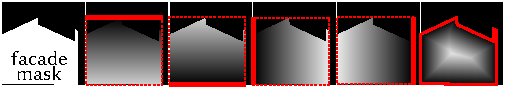
\includegraphics[width=\columnwidth]{images/metrics.pdf}
    \caption{Additional input channels. GANs are conditioned on additional channels that include information about the global context at each pixel. Given a facade/roof mask, we include the distance to the facade boundary and the distance to each bounding box side, making it easy for the network to decide how far it is from the boundary and at what height on the facade.}
    \vspace{-5pt}
    \label{fig:context_info}
\end{figure}

In our experiments, we observed that using this BicycleGAN setup to go directly from inputs to outputs in each step often resulted in implausible global structure, such as misaligned windows or ledges on facades. The limited receptive field of outputs in both the generator and the discriminator constrains coordination between distant output pixels, making it difficult to create globally consistent structure. Increasing the depth of the networks to increase the receptive field alleviates the problem but has a significant resource cost and destabilizes training. We found that conditioning the GANs on additional information about the global context of each pixel was more efficient. More specifically, we conditioned the GANs on five additional channels that are appended to $A$: the distance in real world units to each side of the bounding box and to the nearest boundary of a facade or roof. Examples are shown in Figure~\ref{fig:context_info}.

\begin{figure*}[t!]
    \centering
    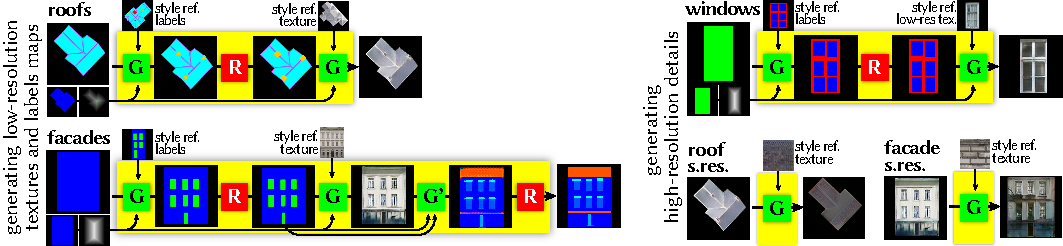
\includegraphics[width=\textwidth]{images/franken_gan.pdf}
    \caption{\systemName details. Each GAN chain (yellow rectangles) consists of several GANs (G) that each perform an image-to-image transformation. GANs are usually conditioned on additional inputs (arrows along the bottom) and are guided by a reference style (arrows along the top). Label outputs are regularized (R) to obtain clean label rectangles. Figure~\ref{fig:overview} shows these chains in context.}
    \label{fig:franken_gan}
\end{figure*}

\begin{figure}[b]
    \centering
    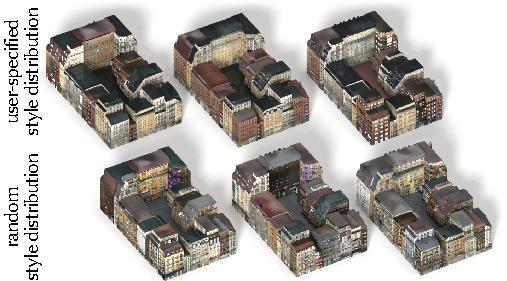
\includegraphics[width=\columnwidth]{images/specified_vs_random_style.pdf}
    \caption{Specifying a style distribution gives control over the generated details. The top row shows three results generated with the same user-specified style distribution, while the bottom row uses the style prior, giving random styles. Note how the buildings in the top row have a consistent style while still allowing for some variation (depending on the variance chosen by the user), while the bottom row does not have a consistent style.}
    \label{fig:specified_vs_random_style}
\end{figure}

\section{FrankenGAN}
\label{sec:franken_gan}

Detail generation is performed by a cascade of textures and label maps, as shown in Figure~\ref{fig:overview}. These are generated by \systemName in several separate chains of GANs, where each GAN is trained and run independently. Splitting up this task into multiple steps rather than training end-to-end has several advantages. First, we can provide more guidance in the form of intermediate objectives, for example window layouts, or low-resolution textures. In our experiments, we show that such intermediate objectives provide a significant advantage over omitting this guidance. While in theory there are several ways to provide intermediate objectives for end-to-end networks, for example by concatenating our current GANs, this would result in extremely large networks, leading to the second advantage of our approach: GAN training is notoriously unstable, and training small GANs is more feasible than training large ones. An end-to-end network with intermediate objectives would need to have a very large generator with multiple discriminators, making stable training difficult achieve. In addition, splitting the network reduces resource costs during training. Instead of a single very large network, we can separately train multiple smaller networks. Note that training a very large network one part at a time
%only keeping part of a very large network in memory during training
%is an option in theory, but in practice it
would require storing and loading parts of the network from disk in each forward and backward pass, which is prohibitive in terms of training times. Finally, using separate GANs, we can regularize intermediate results with operations that are not are not differentiable or would not provide a good gradient signal.

\subsection{Style Control}
\label{sec:style_control}

One difficulty with using separate GANs is achieving stylistically consistent results. For example, windows on the same facade usually have a similar style, as do ledges or window sills. Style control is also necessary beyond single roof or facade textures: adjacent facades on a building usually look similar, and city blocks may have buildings with similar facade and roof styles. A comparison of generated details with and without style control is given in Figure~\ref{fig:specified_vs_random_style}.
%
In \systemName, style can be specified for eight properties: the coarse facade and roof texture, facade and roof texture details, such as brick patterns, the window layout on the facade, the glass pane layout in the windows, the window texture, and the layout of chimneys and windows on a roof. The user can describe the style distribution of a property over a building block with a mixture of isotropic Gaussians in style space $\mathcal{Z}$:
\begin{equation}
    p(Z|\mathbf{S}, \bm{\sigma}) = \sum _{i=1}^{m}\phi_{i}\mathcal{N}(E(S_i),\sigma_{i}),
\end{equation}
where $Z \in \mathcal{Z}$ is the style vector, $\mathcal{N}$ is the normal distribution and the weights $\phi_{i}$ must sum to $1$. $Z$ provides a compact representation of style. We use an eight-dimensional style space in our experiments. The means of the Gaussians are specified by encoding $m$ style reference images $S_i \in \mathbf{S}$ with the encoder described in the previous section. The variance $\bm{\sigma} = (\sigma_1, \dots, \sigma_m)$ specifies the diversity of the generated details and can be adjusted per reference image with a slider. One of these distributions can be specified per property and the styles are sampled independently.

In many cases, however, the styles of different properties are dependent. For example, the color of roofs and facades may be correlated. To specify these dependencies, several sets of property distributions may be specified, each set $\mathcal{S}_i = \{(\mathbf{S}_p, \bm{\sigma}_p)\}_{p=1 \dots 8}$ contains one mixture model per property $p$. For each building, one of these sets is chosen at random. The special case of having a single Gaussian ($m=1$) per property in each set effectively gives a Gaussian mixture model over the \emph{joint} space of all properties, with each set being one component. The user does not need to provide the style for all properties. Any number of properties may be left unspecified, in which case the style vector is sampled from the GAN's style prior, which is a standard normal distribution.


\subsection{Detail Generation}
\label{sec:detail_generation}
\systemName uses five chains of GANs, which can be split into two groups: two chains for generating initial coarse details (textures and label maps) for roofs and facades, and three chains for increasing the resolution given the coarse outputs of the first group. Details of these chains are shown in Figure~\ref{fig:franken_gan}. Most of the chains have intermediate results, which are used for the geometry synthesis that we will describe in Section~\ref{sec:geometry_synthesis}. Each GAN takes an input image and outputs a transformed image. In addition to the input image, all GANs except for the super-resolution networks are conditioned on the scale and context information described in the previous section, making it easier to generate consistent global structure. Each GAN is also guided by a style that is drawn from a distribution, as described above. Figure~\ref{fig:franken_gan} shows reference images $S_i$ that are used to specify the distribution. Images output by GANs are either label maps $L$, or textures $T$. Each label map output by a GAN is passed through a regularizer $R$, denoted by the red rectangles in Figure~\ref{fig:franken_gan}, to produce a clean set of boxes $R(L)$ before being passed to the next step. We now describe each chain in detail. The regularizers are described in Section~\ref{sec:regularizers}.
%For brevity, we will not explicitly describe scale, context and style in each chain, and assume they are included implicitly for each GAN.

%$L_r$ %$T_r$ $L^{\sim}_r$ $L_r = (R_{Lr} \circ G_{Lr})(L^{\sim}_r)$ $T_r = G_{Tr}(L_r)$
\paragraph{Roofs}
The roof chain generates roof detail labels and the coarse roof texture. The chain starts with a coarse label map  of the roof as the input image. This label map includes ridge and valley lines of the roof, which are obtained directly from the mass model. Flat roofs are labeled with a separate color. The first GAN adds chimneys and pitched roof windows. These labels are regularized and then used by the second GAN to generate the coarse roof texture.

\begin{figure}[t]
    \centering
    \includegraphics[width=\columnwidth]{images/super.pdf}
    \caption{Super-resolution. Given inputs (green, magenta), the super-resolution network creates high-quality textures for the walls, while the window GAN chain provides high-quality windows. Note that the window label and window texture networks each run once for every window.}
    \vspace{-5pt}
    \label{fig:super}
\end{figure}

\paragraph{Facades}
The facade chain generates window labels, full facade labels, and the coarse facade texture. Window labels are generated separately from the full labels, since they may be occluded by some of the other labels. The first GAN starts by creating window and door labels from facade boundaries. These are regularized before being used as input in the second GAN to generate the coarse facade texture. The third GAN detects the full set of facade labels from the facade texture, including ledges, window sills, and balconies, which are also regularized to give a cleaner set of labels. The third GAN has a different architecture: since we expect there to be a single correct label map for each facade texture, we do not need style input, which simplifies the GAN to the Pix2Pix architecture~\cite{pix2pix}. Since the window and door labels are known at this point, we also condition this GAN on these labels. Detecting the full label set from the facade texture instead of generating it beforehand and using it as input for the texture generation step is a design choice that we made after experimenting with both variants. Detail outlines in the generated texture tend to follow the input labels very closely, and constraining the details in this way results in unrealistic shapes and reduced variability. For all three GANs, areas occluded by nearby facades are set to the background colour; this ensures that the feature distribution takes into account the nearby geometry.

Since the layout of dormer windows needs to be consistent with the facade layout, we create these windows in the facade chain. More specifically, we extend the input facade mask with a projection of the roof to the facade plane. This allows us to treat the roof as part of the facade and to generate a window layout that extends to the roof. Roof features (chimneys or pitched windows) that intersect dormer windows are removed. 

\paragraph{Windows}
To obtain high-resolution window textures, we apply the window chain to each window separately, using a consistent style. Each window is cut out from the window label map that was generated in the facade chain, and scaled up to the input resolution of the GAN. The steps in the window chain are then similar to those in the roof chain. We generate glass pane labels from the window region, regularize them, and generate the high-resolution window texture from the glass pane labels. %Different from the roof chain, the style of the window texture GAN is not sampled from a given distribution, but is instead encoded from the window patch in the coarse facade texture to maintain consistency with the surrounding facade.
%\paul{do we still use the low-res window texture as style, or is it manually defined?}
% If manual, this needs to be changed here, number of properties increased by 1, and the overview figure should contain an example of a window texture style

\paragraph{Super-resolution}
High-resolution roof and facade textures are obtained with two GANs that are trained to generate texture detail, such as bricks or roof tiles from a given low-resolution input. Roof and facade textures are split into a set of patches that are processed separately. Each patch is scaled up to the input size of the GANs before generating the high-resolution output. Consistency can be maintained by fixing the style for the entire building. The output patches are then assembled to obtain the high-resolution roof and facade textures. Boundaries between patches are blended linearly to avoid seams. Examples are shown in Figure.~\ref{fig:super}. Our interleaved GANs allow us to augment the super-resolution texture map with texture cues from the label maps. For example, window sills are lightened, and roof crests are drawn; these augmentations take the form of drawing the labels in a single colour with a certain alpha. 
\emph{Note that because of the large scale of the super-resolution bitmaps, we explicitly state which figures use these two networks.}


\subsection{Regularizers}
\label{sec:regularizers}
Our GANs are good at producing varied label maps that follow the data distribution in our training set. Alignment between individual elements is, however, usually not perfect. For example, window sills may not be rectangular or have different sizes in adjacent windows, or ledges may not be perfectly straight. Although the discrepancy is usually small, it is still noticeable in the final output. Our multi-step approach allows us to use any non-differentiable (or otherwise) regularization. We exploit domain-specific knowledge to craft simple algorithms to improve the alignment of the label maps. We then provide 3D locations for geometric features. In the following, we describe our regularizers in detail.


\begin{figure}[t!]
    \centering
    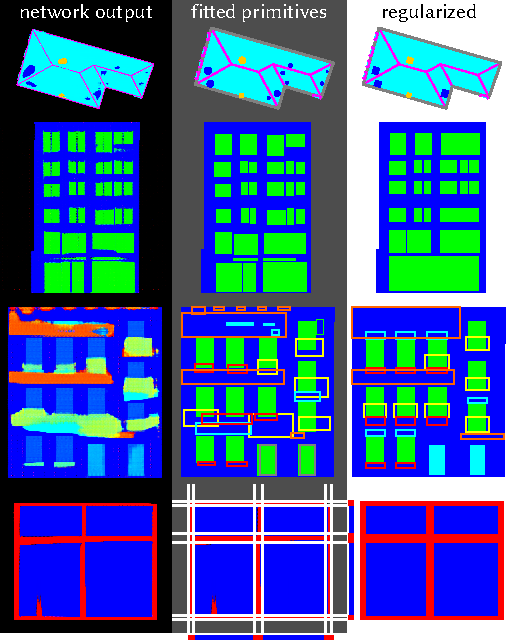
\includegraphics[width=\columnwidth]{images/regularizers.pdf}
    \caption{\changed{Regularization. All our label maps are regularized before being used by the next GAN in the chain.
    %Columns: network outputs (images), fitted primitives (boxes and circles), and regularized results.
    Rows: roof details, facade windows, facade details, and window details (regularized with an outer product). }}
    \vspace{-5pt}
    \label{fig:regularizers}
\end{figure}

%\begin{figure}[t!]
%    \centering
%    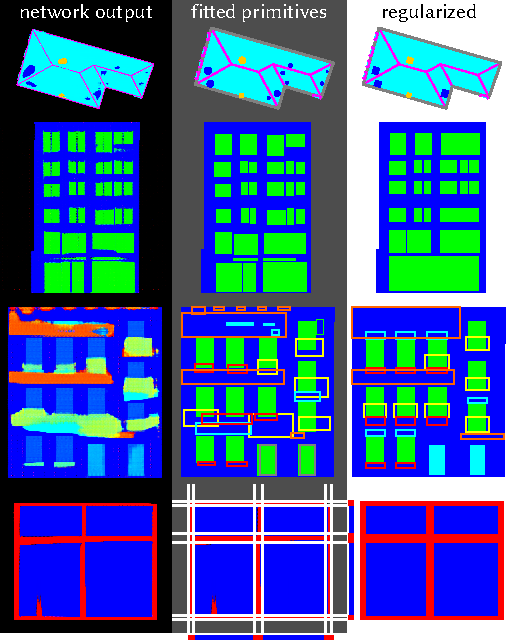
\includegraphics[width=\columnwidth]{images/regularizers.pdf}
%    \caption{Window detail regularization. All our label maps are regularized before being used by the next GAN in the chain. Here, we regularize window glass pane labels using the outer product of two 1D label masks.}
%    \label{fig:regularizers}
%\end{figure}

\paragraph{Roof detail labels}
\changed{Chimneys and pitched roof windows are regularized by fitting circles to the network output. These are then converted to rectangles, which may be oriented to the roof pitch, see Figure~\ref{fig:regularizers}, top row. We take the center of each connected component of a given label and use its area to estimate a circle size. Smaller circles are removed before we convert each to a square. We observe that roof features such as chimneys and roof windows are typically aligned to the roof's slope. We therefore orient the bottom edge of each feature to the gutter of the associated roof pitch.  Finally, we shrink it so that it lies entirely within a single roof pitch and avoids dormer windows.}

\paragraph{Facade window and door labels}
The window and door layout on a facade has to be regularized without removing desirable irregularities introduced by the GAN that reflect the actual data distribution, such as different window sizes on different floors, or multiple overlayed grid layouts. We start by fitting axis-aligned bounding boxes to doors and windows \changed{(see Figure~\ref{fig:regularizers}, second row center). Then we collect a set of properties for each window, including the x and y extents and the spacing between neighbours, over which we perform a mean-shift clustering. We use a square kernel of size 0.4 meters for each property, until convergence or a maximum of 50 mean-shift iterations. This ensures that these properties can have a multi-modal distribution, which preserves desirable irregularities, while also removing small-scale irregularities (see Figure~\ref{fig:regularizers}, second row right).}

\paragraph{Facade detail labels}
Since adjacent details are often not perfectly aligned, we snap nearby details, such as window sills and windows to improve the alignment. We also observed that in the generated label map, the placement of small details such as window sills and moldings is sometimes not coordinated over larger distances on the facade. To improve regularity, we propagate details such as window sills and moldings that are present in more than $50\%$ of the windows in a row to all remaining windows \changed{(see Figure~\ref{fig:regularizers}, third row).}

\paragraph{Window detail labels}
The glass pane layout in a window is usually more regular than the window layout on facades, allowing for a simpler regularization: we transform the label map into a binary glass pane mask and approximate this 2D mask by the outer product of two 1D masks, one for the columns, and one for the rows of the 2D mask. This representation ensures that the mask contains a grid of square glass panes. The two 1D masks are created by taking the mean of the 2D mask in the x- and y-directions, and thresholding them at $0.33$. An example is shown in Figure~\ref{fig:regularizers}, bottom row.

\begin{figure}[t!]
    \centering
    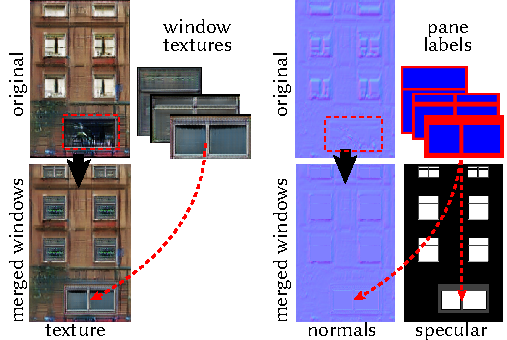
\includegraphics[width=\columnwidth]{images/merge_maps.pdf}
    \caption{Generated window textures and labels are merged back into the facade texture, increasing fidelity of window textures, normals and materials.}
    \label{fig:merge_maps}
\end{figure}

% \subsection{Facade Textures}
% \label{sec:facade_textures}
% \subsection{Roof Textures}
% \label{sec:roof_textures}
% \subsection{Window Textures}
% \label{sec:window_textures}
% \subsection{Facade Super-resolution}
% \label{sec:super_resolution}

\subsection{Geometry Synthesis}
\label{sec:geometry_synthesis}

As output of the five GAN chains, we have high-resolution roof, facade, and window textures, as well as regularized label maps for roof details, facade details, and window panes. These are used to generate the detailed mass model. First, geometry for details is generated procedurally based on the label maps. For details such as window sills and ledges, we use simple extrusions, while balconies and chimneys are generated with small procedural programs to fit the shape given by the label map. 

To apply the generated textures to the detailed mass models, UV maps are generated procedurally along with the geometry. In addition to textures, we also define building materials based on the label maps. Each label is given a set of material properties: windows, for example, are reflective and have high glossiness, while walls are mostly diffuse. To further increase the fidelity of our models, textures and label maps are used to heuristically generate normal maps. The intensity of the generated texture is treated as a height field that allows us to compute normals. While this does not give us accurate normals, it works well in practice to simulate the roughness of a texture. Per-label roughness weights ensure that details such as glass panes still remain flat. Finally, generated window textures and label maps are merged back into the facade textures; an example is given in Figure~\ref{fig:merge_maps}.

\begin{figure*}[t]
    \centering
    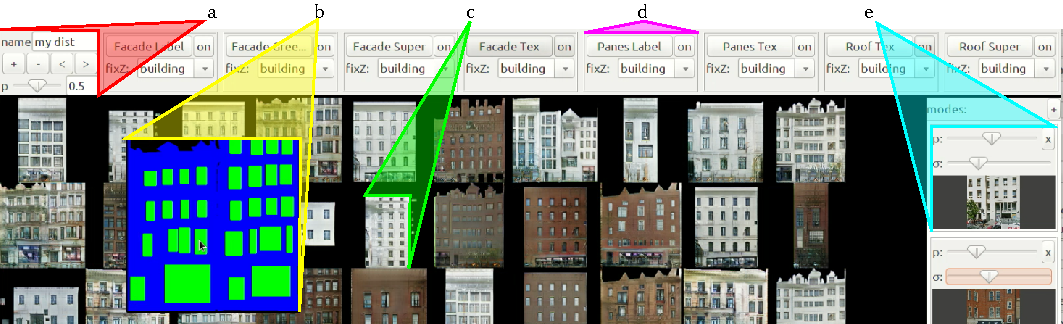
\includegraphics[width=\textwidth]{images/ui_fig.pdf}
    \caption{The distribution designer UI (see supplemental video). Given a style distribution (a), the system continuously shows evaluations of that distribution (c). By clicking on an image, the user can see the network inputs (b). Different networks can be selected (d). The style distribution for any network is a Gaussian mixture model that may have multiple modes (e), the mean of which is given by an exemplar image.}
    \vspace{-5pt}
    \label{fig:ui}
\end{figure*}

\begin{figure*}[t]
    \centering
    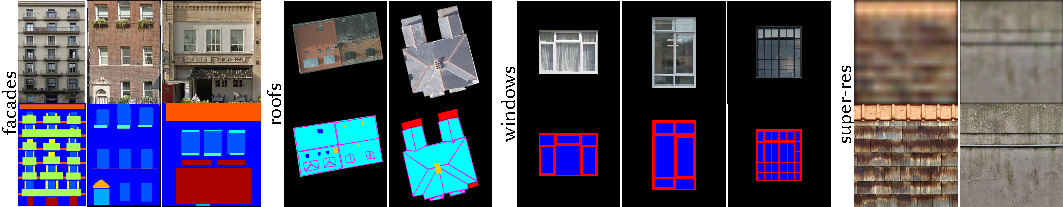
\includegraphics[width=\textwidth]{images/dataset.pdf}
    \caption{Datasets used to train our GANs. We use four datasets of labeled images, a few examples are shown here.}
    \label{fig:dataset}
\end{figure*}

\subsection{User interface}

Our system contains a complete framework for interactively using \systemName. A user may select an urban city block, specify a distribution, and then the system adds the additional geometry and textures to the 3D view. At this point, the user can edit semantic details (such as window locations), while seeing texture updates in real time. Of note is our interface to build our joint distributions (Figure~\ref{fig:ui}), which continually shows the user new examples drawn from the current distribution. The accompanying video demonstrates the user interface.
%\changed{\sout{The source code of our system, and weights for accompanying networks, will be made available online.}}

